\begin{frame}[fragile]
    \frametitle{GTSAM: Georgia Tech Smoothing and Mapping}
    \note{Factor Graphs and GTSAM: A Hands-on Introduction http://hdl.handle.net/1853/45226}
    \note{José Luis Blanco Factor-Gprah Tutorial: https://www.youtube.com/playlist?list=PLOJ3GF0x2_eWtGXfZ5Ne1Jul5L-6Q76Sz}
    \note{GTSAM Tutorial: https://gtsam.org/notes/GTSAM-Concepts.html}

    \begin{itemize}
        \item GTSAM toolbox (GTSAM stands for ``Georgia Tech Smoothing and Mapping'') toolbox is a BSD-licensed C++ library based on factor graphs, developed at the Georgia Institute of Technology by Frank Dellaert and his group.
        \item It provides state of the art solutions to the SLAM and SFM problems, but can also be used to model and solve both simpler and more complex estimation problems.
        \item MATLAB and Python wrappers for rapid prototype development
    \end{itemize}


\begin{lstlisting}[style=bash] 
    https://github.com/borglab/gtsam/blob/develop/python/gtsam/examples/OdometryExample.py
    https://github.com/borglab/gtsam/blob/develop/python/gtsam/examples/Pose2SLAMExample.ipynb
\end{lstlisting}

\end{frame}

\begin{frame}[fragile]
    \frametitle{Modeling Robot Motion}
    \note{Factor Graphs and GTSAM: A Hands-on Introduction http://hdl.handle.net/1853/45226}
    \note{José Luis Blanco Factor-Gprah Tutorial: https://www.youtube.com/playlist?list=PLOJ3GF0x2_eWtGXfZ5Ne1Jul5L-6Q76Sz}
    \note{GTSAM Tutorial: https://gtsam.org/notes/GTSAM-Concepts.html}

    \note{https://github.com/borglab/gtsam/blob/develop/python/gtsam/examples/OdometryExample.py}


    \scriptsize

    \begin{figure}[!h]
        
\includegraphics[width=0.5\textwidth]{./images/gtsam/factor_graph_odometry.pdf}
    \end{figure}

\begin{lstlisting}[style=python] 
# Create noise models
ODOMETRY_NOISE = gtsam.noiseModel.Diagonal.Sigmas(np.array([0.2, 0.2, 0.1]))
PRIOR_NOISE = gtsam.noiseModel.Diagonal.Sigmas(np.array([0.3, 0.3, 0.1]))
\end{lstlisting}

\begin{lstlisting}[style=python] 
# Create an empty nonlinear factor graph
graph = gtsam.NonlinearFactorGraph()

# Add a prior on the first pose, setting it to the origin
# A prior factor consists of a mean and a noise model (covariance matrix)
priorMean = gtsam.Pose2(0.0, 0.0, 0.0)  # prior at origin
graph.add(gtsam.PriorFactorPose2(1, priorMean, PRIOR_NOISE))

# Add odometry factors
odometry = gtsam.Pose2(2.0, 0.0, 0.0)
# For simplicity, we will use the same noise model for each odometry factor
# Create odometry (Between) factors between consecutive poses
graph.add(gtsam.BetweenFactorPose2(1, 2, odometry, ODOMETRY_NOISE))
graph.add(gtsam.BetweenFactorPose2(2, 3, odometry, ODOMETRY_NOISE))
print("\nFactor Graph:\n{}".format(graph))
\end{lstlisting}

\end{frame}

\begin{frame}[fragile]
    \frametitle{Modeling Robot Motion}
    \note{Factor Graphs and GTSAM: A Hands-on Introduction http://hdl.handle.net/1853/45226}
    \note{José Luis Blanco Factor-Gprah Tutorial: https://www.youtube.com/playlist?list=PLOJ3GF0x2_eWtGXfZ5Ne1Jul5L-6Q76Sz}
    \note{GTSAM Tutorial: https://gtsam.org/notes/GTSAM-Concepts.html}

    \note{https://github.com/borglab/gtsam/blob/develop/python/gtsam/examples/OdometryExample.py}


    \scriptsize

    \begin{figure}[!h]
        
\includegraphics[width=0.5\textwidth]{./images/gtsam/factor_graph_odometry.pdf}
    \end{figure}

    Terminal Output:
\begin{lstlisting}[style=bash] 
Factor Graph:
NonlinearFactorGraph: size: 3

Factor 0: PriorFactor on 1
    prior mean:  (0, 0, 0)
    noise model: diagonal sigmas [0.3; 0.3; 0.1];

Factor 1: BetweenFactor(1,2)
    measured:  (2, 0, 0)
    noise model: diagonal sigmas [0.2; 0.2; 0.1];

Factor 2: BetweenFactor(2,3)
    measured:  (2, 0, 0)
    noise model: diagonal sigmas [0.2; 0.2; 0.1];
\end{lstlisting}

\end{frame}

\begin{frame}
    \frametitle{Modeling Robot Motion}
    \note{Factor Graphs and GTSAM: A Hands-on Introduction http://hdl.handle.net/1853/45226}
    \note{José Luis Blanco Factor-Gprah Tutorial: https://www.youtube.com/playlist?list=PLOJ3GF0x2_eWtGXfZ5Ne1Jul5L-6Q76Sz}
    \note{GTSAM Tutorial: https://gtsam.org/notes/GTSAM-Concepts.html}

    \note{https://github.com/borglab/gtsam/blob/develop/python/gtsam/examples/OdometryExample.py}

    \begin{figure}[!h]
        
\includegraphics[width=0.5\textwidth]{./images/gtsam/factor_graph_odometry.pdf}
    \end{figure}

    \begin{itemize}
        \item The factor graph and its embodiment in code specify the joint probability distribution $P(X \mid Z)$ over the entire trajectory $ X = \{ x_1,x_2,x_3 \}$ of the robot, rather than just the last pose.
        \item A factor graph in GTSAM is just the specification of the probability density $P(X \mid Z)$, and the corresponding \textbf{FactorGraph} class and its derived classes do not ever contain a ``solution''. Rather, there is a separate type \textbf{Values} that is used to specify specific values for (in this case) $x_1$, $x_2$, and $x_3$, which can then be used to evaluate the probability (or, more commonly, the error) associated with particular values.
        \item Think a factor graph as a function to be applied to values --as the notation $f(X) \propto P(X \mid Z)$ implies-- rather than as an object to be modified.
    \end{itemize}

\end{frame}

\begin{frame}[fragile]
    \frametitle{Non Linear Optimization in GTSAM}
    \note{Factor Graphs and GTSAM: A Hands-on Introduction http://hdl.handle.net/1853/45226}
    \note{José Luis Blanco Factor-Gprah Tutorial: https://www.youtube.com/playlist?list=PLOJ3GF0x2_eWtGXfZ5Ne1Jul5L-6Q76Sz}
    \note{GTSAM Tutorial: https://gtsam.org/notes/GTSAM-Concepts.html}
    \note{https://github.com/borglab/gtsam/blob/develop/python/gtsam/examples/OdometryExample.py}

    \scriptsize

    \begin{figure}[!h]
        
\includegraphics[width=0.5\textwidth]{./images/gtsam/factor_graph_odometry.pdf}
    \end{figure}

    \begin{itemize}
        \item  The listing below creates a Values instance, and uses it as the initial estimate to find the maximum a-posteriori (MAP) assignment for the trajectory $X$:
    
\begin{lstlisting}[style=python] 
# Create the data structure to hold the initialEstimate estimate to the solution
# For illustrative purposes, these have been deliberately set to incorrect values
initial = gtsam.Values()
initial.insert(1, gtsam.Pose2(0.5, 0.0, 0.2))
initial.insert(2, gtsam.Pose2(2.3, 0.1, -0.2))
initial.insert(3, gtsam.Pose2(4.1, 0.1, 0.1))
print("\nInitial Estimate:\n{}".format(initial))

# optimize using Levenberg-Marquardt optimization
params = gtsam.LevenbergMarquardtParams()
optimizer = gtsam.LevenbergMarquardtOptimizer(graph, initial, params)
result = optimizer.optimize()
print("\nFinal Result:\n{}".format(result))
\end{lstlisting}
        
        \item Odometry factors $f_{1}(x_1, x_2; o_1)$ and $f_{2}(x_2, x_3; o_2)$ are non-linear, as they involve the orientation of the robot.
        \item The optimization class (\textbf{NonlinearFactorGraph}) linearizes this graph, possibly multiple times, to minimize the non-linear squared error specified by the factors.
    \end{itemize}

\end{frame}

\begin{frame}[fragile]
    \frametitle{Non Linear Optimization in GTSAM}
    \note{Factor Graphs and GTSAM: A Hands-on Introduction http://hdl.handle.net/1853/45226}
    \note{José Luis Blanco Factor-Gprah Tutorial: https://www.youtube.com/playlist?list=PLOJ3GF0x2_eWtGXfZ5Ne1Jul5L-6Q76Sz}
    \note{GTSAM Tutorial: https://gtsam.org/notes/GTSAM-Concepts.html}
    \note{https://github.com/borglab/gtsam/blob/develop/python/gtsam/examples/OdometryExample.py}

    \scriptsize

    \begin{figure}[!h]
        
\includegraphics[width=0.5\textwidth]{./images/gtsam/factor_graph_odometry.pdf}
    \end{figure}
\begin{lstlisting}[style=bash] 
Initial Estimate:
Values with 3 values:
Value 1: (gtsam::Pose2)
(0.5, 0, 0.2)
Value 2: (gtsam::Pose2)
(2.3, 0.1, -0.2)
Value 3: (gtsam::Pose2)
(4.1, 0.1, 0.1)

Final Result:
Values with 3 values:
Value 1: (gtsam::Pose2)
(7.46978305e-16, -5.34409097e-16, -1.78381861e-16)
Value 2: (gtsam::Pose2)
(2, -1.09236636e-15, -2.48671177e-16)
Value 3: (gtsam::Pose2)
(4, -1.70076056e-15, -2.50943862e-16)
\end{lstlisting}

    \begin{itemize}
        \item It can be seen that, subject to very small tolerance, the ground truth solution $x_1 = (0,0,0)$, $x_2 = (2,0,0)$, and $x_3 = (4,0,0)$ is recovered.
    \end{itemize}

\end{frame}


\begin{frame}[fragile]
    \frametitle{Full Posterior Inference}
    \note{Factor Graphs and GTSAM: A Hands-on Introduction http://hdl.handle.net/1853/45226}
    \note{José Luis Blanco Factor-Gprah Tutorial: https://www.youtube.com/playlist?list=PLOJ3GF0x2_eWtGXfZ5Ne1Jul5L-6Q76Sz}
    \note{GTSAM Tutorial: https://gtsam.org/notes/GTSAM-Concepts.html}
    \note{https://github.com/borglab/gtsam/blob/develop/python/gtsam/examples/OdometryExample.py}

    \scriptsize

    \begin{figure}[!h]
        
\includegraphics[width=0.5\textwidth]{./images/gtsam/factor_graph_odometry.pdf}
    \end{figure}

    \begin{itemize}
        \item GTSAM can also be used to calculate the covariance matrix for each pose after incorporating the information from all measurements $Z$. Recognizing that the factor graph encodes the \textbf{posterior density} $P(X \mid Z)$, the mean $\mu$ together with the covariance $\Sigma$ for each pose $x$ approximate the \textbf{marginal posterior density} $P(x \mid Z)$. Note that this is just an approximation, as even in this simple case the odometry factors are actually non-linear in their arguments, and GTSAM only computes a Gaussian approximation to the true underlying posterior.
    \end{itemize}

    \tiny

\begin{lstlisting}[style=python] 
# Calculate and print marginal covariances for all variables
marginals = gtsam.Marginals(graph, result)
for i in range(1, 4):
    print("X{} covariance:\n{}\n".format(i,
                                        marginals.marginalCovariance(i)))
\end{lstlisting}

\begin{lstlisting}[style=bash] 
X1 covariance:
[[9.00000000e-02 3.19488667e-33 2.83989926e-33]
    [3.19488667e-33 9.00000000e-02 2.55795385e-17]
    [2.83989926e-33 2.55795385e-17 1.00000000e-02]]

X2 covariance:
[[1.30000000e-01 1.21229814e-18 6.06149069e-19]
    [1.21229814e-18 1.70000000e-01 2.00000000e-02]
    [6.06149069e-19 2.00000000e-02 2.00000000e-02]]

X3 covariance:
[[1.70000000e-01 8.63317012e-18 2.69082491e-18]
    [8.63317012e-18 3.70000000e-01 6.00000000e-02]
    [2.69082491e-18 6.00000000e-02 3.00000000e-02]]
\end{lstlisting}

\note{What we see is that the marginal covariance $P(x_1 \mid Z)$ on $x_1$ is simply the prior knowledge on $x_1$, but as the robot moves the uncertainty in all dimensions grows without bound, and the y and $\theta$ components of the pose become (positively) correlated.
An important fact to note when interpreting these numbers is that covariance matrices are given in relative coordinates, not absolute coordinates. This is because internally GTSAM optimizes for a change with respect to a linearization point, as do all nonlinear optimization libraries.}

\end{frame}

\begin{frame}
    \frametitle{Full Posterior Inference}
    \note{Factor Graphs and GTSAM: A Hands-on Introduction http://hdl.handle.net/1853/45226}
    \note{José Luis Blanco Factor-Gprah Tutorial: https://www.youtube.com/playlist?list=PLOJ3GF0x2_eWtGXfZ5Ne1Jul5L-6Q76Sz}
    \note{GTSAM Tutorial: https://gtsam.org/notes/GTSAM-Concepts.html}
    \note{https://github.com/borglab/gtsam/blob/develop/python/gtsam/examples/OdometryExample.py}

    \begin{figure}[!h]
        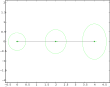
\includegraphics[width=0.6\textwidth]{./images/gtsam/gtsam_odometry.pdf}
    \end{figure}

\end{frame}


\begin{frame}
    \frametitle{Loop Closure Constraints}
    \note{Factor Graphs and GTSAM: A Hands-on Introduction http://hdl.handle.net/1853/45226}
    \note{José Luis Blanco Factor-Gprah Tutorial: https://www.youtube.com/playlist?list=PLOJ3GF0x2_eWtGXfZ5Ne1Jul5L-6Q76Sz}
    \note{GTSAM Tutorial: https://gtsam.org/notes/GTSAM-Concepts.html}
    \note{https://github.com/borglab/gtsam/blob/develop/python/gtsam/examples/Pose2SLAMExample.ipynb}

    \begin{figure}[!h]
        
\includegraphics[width=0.8\textwidth]{./images/gtsam/factor_graph_loop_closure.pdf}
    \end{figure}

\end{frame}

\begin{frame}[fragile]
    \frametitle{Loop Closure Constraints}
    \note{Factor Graphs and GTSAM: A Hands-on Introduction http://hdl.handle.net/1853/45226}
    \note{José Luis Blanco Factor-Gprah Tutorial: https://www.youtube.com/playlist?list=PLOJ3GF0x2_eWtGXfZ5Ne1Jul5L-6Q76Sz}
    \note{GTSAM Tutorial: https://gtsam.org/notes/GTSAM-Concepts.html}
    \note{https://github.com/borglab/gtsam/blob/develop/python/gtsam/examples/Pose2SLAMExample.ipynb}


    \scriptsize

\begin{lstlisting}[style=python] 
# Create a factor graph container
graph = gtsam.NonlinearFactorGraph()

# Add a prior on the first pose (key 1)
graph.add(gtsam.PriorFactorPose2(1, gtsam.Pose2(0, 0, 0), PRIOR_NOISE))

# Add odometry factors (Between Factors)
# Between poses 1 and 2:
graph.add(gtsam.BetweenFactorPose2(1, 2, gtsam.Pose2(2, 0, 0), ODOMETRY_NOISE))
# Between poses 2 and 3:
graph.add(gtsam.BetweenFactorPose2(2, 3, gtsam.Pose2(2, 0, math.pi / 2), ODOMETRY_NOISE))
# Between poses 3 and 4:
graph.add(gtsam.BetweenFactorPose2(3, 4, gtsam.Pose2(2, 0, math.pi / 2), ODOMETRY_NOISE))
# Between poses 4 and 5:
graph.add(gtsam.BetweenFactorPose2(4, 5, gtsam.Pose2(2, 0, math.pi / 2), ODOMETRY_NOISE))

# Add the loop closure constraint
# This factor connects pose 5 back to pose 2
# The measurement is the expected relative pose from 5 to 2
graph.add(gtsam.BetweenFactorPose2(5, 2, gtsam.Pose2(2, 0, math.pi / 2), ODOMETRY_NOISE))
\end{lstlisting}

\end{frame}

\begin{frame}
    \frametitle{Loop Closure Constraints}
    \note{Factor Graphs and GTSAM: A Hands-on Introduction http://hdl.handle.net/1853/45226}
    \note{José Luis Blanco Factor-Gprah Tutorial: https://www.youtube.com/playlist?list=PLOJ3GF0x2_eWtGXfZ5Ne1Jul5L-6Q76Sz}
    \note{GTSAM Tutorial: https://gtsam.org/notes/GTSAM-Concepts.html}
    \note{https://github.com/borglab/gtsam/blob/develop/python/gtsam/examples/Pose2SLAMExample.ipynb}

    \begin{figure}[!h]
        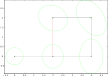
\includegraphics[width=0.7\textwidth]{./images/gtsam/gtsam_loop_closure.pdf}
    \end{figure}

\end{frame}

\begin{frame}
    \frametitle{Landmark-based SLAM}
    \note{Factor Graphs and GTSAM: A Hands-on Introduction http://hdl.handle.net/1853/45226}
    \note{José Luis Blanco Factor-Gprah Tutorial: https://www.youtube.com/playlist?list=PLOJ3GF0x2_eWtGXfZ5Ne1Jul5L-6Q76Sz}
    \note{GTSAM Tutorial: https://gtsam.org/notes/GTSAM-Concepts.html}
    \note{https://github.com/borglab/gtsam/blob/develop/python/gtsam/examples/PlanarSLAMExample.ipynb}

    \begin{figure}[!h]
        
\includegraphics[width=0.6\textwidth]{./images/gtsam/factor_graph_landmark_based_slam.pdf}
    \end{figure}

\end{frame}

\begin{frame}[fragile]
    \frametitle{Loop Closure Constraints}
    \note{Factor Graphs and GTSAM: A Hands-on Introduction http://hdl.handle.net/1853/45226}
    \note{José Luis Blanco Factor-Gprah Tutorial: https://www.youtube.com/playlist?list=PLOJ3GF0x2_eWtGXfZ5Ne1Jul5L-6Q76Sz}
    \note{GTSAM Tutorial: https://gtsam.org/notes/GTSAM-Concepts.html}
    \note{https://github.com/borglab/gtsam/blob/develop/python/gtsam/examples/Pose2SLAMExample.ipynb}


    \scriptsize

\begin{lstlisting}[style=python]
# Create noise models with specified standard deviations (sigmas).
PRIOR_NOISE = gtsam.noiseModel.Diagonal.Sigmas(np.array([0.3, 0.3, 0.1]))
ODOMETRY_NOISE = gtsam.noiseModel.Diagonal.Sigmas(np.array([0.2, 0.2, 0.1]))
# Measurement noise (bearing, range) - sigmas = [0.1rad, 0.2m]
MEASUREMENT_NOISE = gtsam.noiseModel.Diagonal.Sigmas(np.array([0.1, 0.2]))

# Create an empty nonlinear factor graph
graph = gtsam.NonlinearFactorGraph()

# Add a prior on pose X(1) at the origin.
graph.add(gtsam.PriorFactorPose2(X(1), gtsam.Pose2(0.0, 0.0, 0.0), PRIOR_NOISE))

# Add odometry factors between X(1),X(2) and X(2),X(3), respectively.
# The measurement is the relative motion: Pose2(dx, dy, dtheta).
graph.add(gtsam.BetweenFactorPose2(X(1), X(2), gtsam.Pose2(2.0, 0.0, 0.0), ODOMETRY_NOISE))
graph.add(gtsam.BetweenFactorPose2(X(2), X(3), gtsam.Pose2(2.0, 0.0, 0.0), ODOMETRY_NOISE))

# Add Range-Bearing measurements to two different landmarks L(1) and L(2).
# Measurements are Bearing (gtsam.Rot2) and Range (float).
graph.add(gtsam.BearingRangeFactor2D(X(1), L(1), gtsam.Rot2.fromDegrees(45), np.sqrt(4.0+4.0), MEASUREMENT_NOISE))
graph.add(gtsam.BearingRangeFactor2D(X(2), L(1), gtsam.Rot2.fromDegrees(90), 2.0, MEASUREMENT_NOISE))
graph.add(gtsam.BearingRangeFactor2D(X(3), L(2), gtsam.Rot2.fromDegrees(90), 2.0, MEASUREMENT_NOISE))
\end{lstlisting}

\end{frame}

\begin{frame}
    \frametitle{Landmark-based SLAM}
    \note{Factor Graphs and GTSAM: A Hands-on Introduction http://hdl.handle.net/1853/45226}
    \note{José Luis Blanco Factor-Gprah Tutorial: https://www.youtube.com/playlist?list=PLOJ3GF0x2_eWtGXfZ5Ne1Jul5L-6Q76Sz}
    \note{GTSAM Tutorial: https://gtsam.org/notes/GTSAM-Concepts.html}
    \note{https://github.com/borglab/gtsam/blob/develop/python/gtsam/examples/PlanarSLAMExample.ipynb}

    \begin{figure}[!h]
        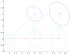
\includegraphics[width=0.6\textwidth]{./images/gtsam/gtsam_landmark_based_slam.pdf}
    \end{figure}

\end{frame}